\chapter{A Language for Metamodelling}
\label{xmofchapter}

\section{Introduction}

In order to be able to construct models of languages, a modelling
language is required. This language is known as a {\em
metamodelling language}. A metamodelling language should provide
the ability to capture the key features of a modelling language,
including its syntax and semantics in a unified and platform
independent way. This chapter introduces an object-oriented
metamodelling language called XMOF (eXecutable MOF) that does just
this. XMOF is an extension to existing standards for metamodelling
such as MOF, OCL and QVT that is rich enough to address all the
requirements of metamodelling. This will form the foundation for
exploring metamodelling throughout the rest of this book.

\section{Requirements of a Metamodelling Language}

Before introducing XMOF, it is important to understand some of the
key requirements of a metamodelling language.

Firstly, as described in the previous chapter, a metamodel should
capture all the essential features of a modelling language. Thus,
a metamodelling language should provide modelling concepts that
can capture the abstract syntax, concrete syntax and semantics of
a language. In addition, it should provide facilities for
manipulating metamodels, including the ability to map them to
other metamodels and extend metamodels to support new language
definitions.

Secondly, a metamodelling language should itself be completely
described by its metamodel, thus ensuring that the language is
self defined and complete, and enabling its definition to be
rapidly reused to create new language metamodels.

Finally, to gain maximum flexibility, a metamodelling language
must be platform independent. In other words, the resulting
metamodels should be self sufficient and independent of
implementation specific descriptions of the language being
modelled. Thus, reliance on the implementation of the language's
behaviour in an external programming language or the assumption
that there will be an external database that manages object
creation and persistence is completely avoided.

\subsection{XMOF}

The metamodelling language presented in this chapter aims to
provide a rich environment for language design that supports the
key requirements of a metamodelling language. This language,
called XMOF, combines and extends a number of standard
object-oriented modelling facilities to provide a minimal, but
expressive, platform independent language for metamodelling. XMOF
includes the following features:

\begin{itemize}

\item Support for standard OO modelling concepts such as packages, classes, and
associations to describe language concepts and their relationship to one another.

\item A constraint language, which can used to describe well-formedness rules.

\item A set of action primitives, which can be used to capture the behavioural
semantics of a language. This turns XMOF into a meta-programming
language.

\item A language for expressing mappings (both uni-directional and bi-directional)
between languages and language components.

\item A concrete syntax language which can be used to model the concrete syntax of
any modelling language.

\item A generic metamodel framework, which supports standard plug-points and machinery for
expressing model element instantiation, execution, expression evaluation and reflection.

\item Conformance to the golden-braid metamodel architecture
described in section \ref{goldenbraid}, ensuring that the
language, including its semantics is completely self describing.

\end{itemize}

The following sections present an overview of the key features of
XMOF. This is not a full definition, but will reference fuller
descriptions of the components of the language where appropriate.

\section{XMOF Features}

\subsection{OO modelling concepts}

XMOF provides the standard OO modelling concepts that are
supported by MOF and UML, including packages, classes and
associations. These are  visualised using class diagrams. Figure
\ref{classDiagram} shows an example of a class diagram of a simple
model consisting of a package with a number of classes and
associations. This model describes a simple StateMachine, where a
StateMachine contains States and Transitions, and Transitions have
source and target states.

\begin{figure}[htb]
\begin{center}
\includegraphics[width=11cm]{XMOF/figures/classDiagramExample}
\caption{An example of a class diagram}
\label{classDiagram}
\end{center}
\end{figure}

XMOF also provides a concrete syntax for packages and classes. The
equivalent concrete representation of the StateMachine class
diagram shown in figure \ref{classDiagram} is shown below.

\small
\begin{verbatim}
1 @Package StateMachines
2    @Class isAbstract Named
3      @Attribute name : String end
4    end
5    @Class StateMachine extends Named
6      @Attribute states : Set(State) end
7      @Attribute transitions : Set(Transition) end
8      @Attribute startingState : State end
9    end
10   @Class State extends Named
11   end
12   @Class Transition extends Named
13     @Attribute source : State end
14     @Attribute target : State end
15   end
16 end
\end{verbatim}

\normalsize

Here, line 1 shows the start of a package named StateMachine,
which contains all the sub-definitions relating to StateMachines.

Line 2 contains the start of a class definition for the class
Named,  which is an abstract class for a named element. Line 5 is
the start of the definition of the StateMachine class. It defines
two attributes named states and transitions, whose types are
Set(State) and Set(Transition). These types correspond to the "*"
multiplicity of the equivalent association ends in the class
diagram.

Lines 10 and 12 are the start of the State and Transition class
definitions. Both these classes specialise the class Named, and
therefore inherit a name attribute. A Transition has two attributes
source and target, which are of type State. The fact that they are
single valued reflects the multiplicity of the equivalent
association ends in the class diagram.

As chapter \ref{concretechapter} will show, the concrete
representation of a modelling language should be clearly
distinguished from its abstract syntax representation. Here, two
different concrete syntaxes are being used to capture the same
information.

\subsection{Imports}

Just as in UML and MOF, a package can be imported into another
package using import. The result is that all referenceable
elements in the imported package can be referenced by elements in
the importing package. Consider the following package:

\small
\begin{verbatim}
@Package X
  @Class Y end
end

@Package A imports X
  @Class B
    @Attribute b : Y end
  end
end
\end{verbatim}
\normalsize

Because the package A imports the package X, then elements in the
package X can be referenced without the need to provide a full
path name.

In addition, XMOF packages can import parsers. Once a parser has
been imported, the syntax and semantics of the language it
supports is immediately available. Thus, the developer can pick
and mix languages that best fit the problem domain. This
capability is an essential part of the flexibility offered by
XMOF's meta-programming environment.

\subsection{Constraints}

It is often necessary to make well-formedness statements about
concepts in a model.  These statements are often made informally,
for example in the context of figure \ref{classDiagram} it might
be useful to specify that \emph{all transitions have unique names
within a state machine}. A constraint language provides a means of
succinctly and unambiguously expressing complex well-formedness
rules. For example the well-formedness statement mentioned above
can be added to the class StateMachine in the following way:

\small
\begin{verbatim}
context StateMachines::StateMachine
  @Constraint NoTwoTransitionsWithTheSameName
    self.transitions->forAll(t1 |
      self.transition->forAll(t2 |
        t1.name = t2.name implies t1 = t2))
  end
\end{verbatim}
\normalsize

Another well-formedness rule requires that the starting state must
be one of the states of the state machine:

\small
\begin{verbatim}
context StateMachines::StateMachine
  @Constraint ValidStartingState
    not self.states->isEmpty implies
      self.states->includes(self.startingState)
  end
\end{verbatim}
\normalsize

The constraint language used in XMOF is OCL \cite{Warmer}. The
primary difference between the OCL used here and the standard OCL
language is in the use of a different syntax for declarations. In
this case ''@Constraint'' is used as opposed to the ''inv:''
declaration used in standard OCL. The reasons for this choice will
become apparent later when we consider the need for a flexible
parsing language.

\subsection{Queries}

OCL can be used to write queries. A query is used to produce a
value in the context of a current object state; it does not cause
any side effects. The following is an example of a query:

\small
\begin{verbatim}
@Class StateMachines
  @Operation getState(n:String):State
    self.states->select(s | s.name = n)->sel
  end
end
\end{verbatim}
\normalsize

This will filter the states of a state machine, selecting those
states whose name matches the string n. Here, sel, is an in-built
operation, which selects a single element from a collection. This
is required in order to return a single State. Again, note that
the declaration of a query differs from that in the OCL standard.

\noindent Another example of query returns true if there exists a
state with the name, n:

\small
\begin{verbatim}
@Class StateMachines
  @Operation isState(n:String):Boolean
    self.states->exists(s | s.name = n)
  end
end
\end{verbatim}
\normalsize

\subsection{Actions and XOCL}

OCL is by design a static language and does not change the state
of objects it refers to.  In some situations this is a good thing
because it guarantees side-effect free evaluation.  However this
limitation makes it very difficult to describe operational
behaviour in a way which can be readily executed.  Standard OCL
does provide pre-/post- conditions as a way of specifying the
effect of an operation, however in general these cannot be
executed.

A better approach is to augment OCL with action primitives. The
XOCL (eXecutable OCL) language extends OCL with a number of key
behaviour primitives. This is a essential step towards making XMOF
a true meta-programming environment.

An example of the application of actions in XOCL can be seen in
the state machine of figure \ref{classDiagram}. If it was required
to add new states to the state machine dynamically then the
following XOCL statement can be written:

\small
\begin{verbatim}
context StateMachines
  @Operation addState(name:String)
    self.states := self.states->including(State(name))
  end
end
\end{verbatim}
\normalsize

New instances of classes can be created by declaring the class as
an operation. In this example a new instance of a State is created
by the declaration State(). The resulting object is then assigned
to the set of states that includes the new state using the
assignment expression \emph{:=}. It is important to recognise that
\emph{:=} and \emph{new} have an imperative semantics and (given
an appropriate implementation) can be executed.

In the above example, the State() operation takes an
initialisation value, which is the name of the state that is to be
created. To handle initialisation parameters, a special operation
called a constructor is provided. It takes a sequence of values as
an argument, which are then used to intialise the object's slots.
In the case of the state machine, three contructors are required,
one for each concrete class. The first intialises the name of a
state, the second assigns a name, and a source and target state to
a transition, and the third initialises a new state machine with a
starting state, set of transitions, and set of states. Note, that
if the body of the constructor is empty, the default action is to
set the attribute values (slots) of the created object with the
values of the parameters.

\small
\begin{verbatim}
context State
  @Constructor(name)
  end

context Transition
  @Constructor(name,source,target)
  end

context StateMachine
  @Constructor(name,source,target)
  end
\end{verbatim}
\normalsize

The body of the next example illustrates how OCL conditional
expressions and logical operators can be combined with XOCL
actions to define the operation of adding a transition. This
operation takes the name of the new transition and the name of a
source and target state. The isState() query is then used to check
that the states belong to the StateMachine before creating a
transition between them. The last line of the if statement shows
how XOCL deals with the printing of strings to the terminal.

\small
\begin{verbatim}
context StateMachines @Operation
addTransition(name:String,source:String,target:String)
  if self.isState(source) and self.isState(target) then
    self.transitions := self.transitions->
      including(Transition(name,s,t))
  else
    "Invalid State in addTransition()".println()
  end
end
\end{verbatim}
\normalsize

As this example show, augmenting OCL with a small number of action
primitives results in a powerful and expressive programming
language. Furthermore, as we will see in later chapters of this
book, because the language works at the XMOF level, it also
provides a rich meta-programming environment that can be used to
construct powerful modelling facilities such as model simulators,
execution engines and compilers. Indeed, it is sufficiently
expressive to enable a complete definition of all the languages in
this book to be constructed.

\subsection{Snapshots}

A useful notation for visually representing the instances of a
metamodel is a snapshot - a notation popularised by the Catalysis
method \cite{Catalysis}. A snapshot shows objects, the values of
their slots (instances of attributes) and links (instances of
associations). A snapshot of a metamodel will thus show objects
and links that are instances of elements in the metamodel. The
example shown in figure \ref{snapshotExample} is a snapshot of the
StateMachine metamodel, and shows an instance of a StateMachine
containing three states and two transitions.

\begin{figure}[htb]
\begin{center}
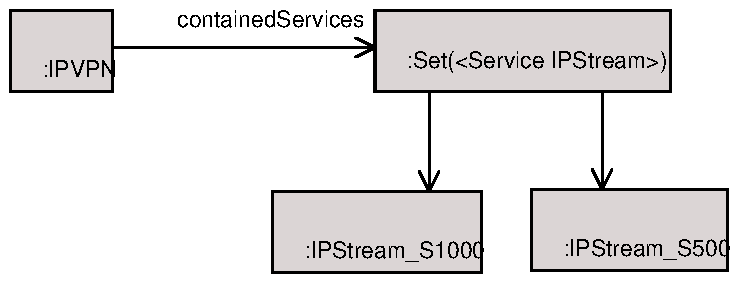
\includegraphics[width=11cm]{XMOF/figures/snapshot.pdf}
\caption{A snapshot showing an instance of the statemachine metamodel}
\label{snapshotExample}
\end{center}
\end{figure}

\subsection{Mappings}

Chapter \ref{mddchapter} highlighted the fact that many languages
are used to design systems from a multitude of perspectives. There
must exist relationships between the perspectives in order to
understand what one model means in terms of another.  These
relationships are implemented by a mapping language which
specifies how we can translate one language into another.  The
mapping language used, XMap, is a declarative, executable language
based on pattern matching. Whilst this language can be viewed as a
XMOF plug-in (as opposed to a core part of the XMOF language), it
is nevertheless important for its ability express mappings in an
intuitive, yet ultimately implementable way.

To illustrate the use of XMap, figure \ref{cppExample} shows a
simple model of {C++} classes which will be used as the target of a
mapping from a state machine.

\begin{figure}[htb]
\begin{center}
\includegraphics[width=11cm]{XMOF/figures/cppExample}
\caption{A simple model of C++ classes}
\label{cppExample}
\end{center}
\end{figure}

A {C++} class is a namespace for its attributes and operations
(methods). An attribute has a type, and for the purposes of this
example, its type may either be another class or an enumeration
type. An enumeration type has a value, which is the sequence of
strings in the enumeration. An operation has a name and a body,
which contains a simple string representation of the body of the
operation.

A mapping from from the StateMachine model in figure
\ref{classDiagram} to the {C++} in \ref{cppExample} can be
defined. This maps a StateMachine to a {C++} class, where each
state in the state machine is mapped to a value in an enumerated
type called STATE. Each transition in the state machine is mapped
to a {C++} operation with the same name and a body, which changes
the state attribute to the target of the transition.

The mapping can be modelled in XMap as shown in figure
\ref{mapping}.  The arrows represent mappings between elements of
the two languages. The first mapping, SM2Class, maps a state
machine to a C++ class. The second mapping, Transition2Op, maps a
transition to an operation.

\begin{figure}[htb]
\begin{center}
\includegraphics[width=11cm]{XMOF/figures/cppMapping}
\caption{A mapping between state machines and C++ classes}
\label{mapping}
\end{center}
\end{figure}

In order to describe the details of the mapping, XMap uses a
textual  mapping language based on pattern matching. Working
backwards, the definition of the mapping between a transition and
an operation is as follows:

\small
\begin{verbatim}
@Map Transition2Op
  @Clause Transition2Op
    Transition
      [name = N,
       target = T]
    when true
    do
    Operation
      [name = N,
       body = B]
    where
      B = "state = " + T.name
  end
end
\end{verbatim}
\normalsize

A mapping consists of a collection of clauses, which are pattern
matches between source and target objects. Whenever a source object
is successfully matched to the input of the mapping, the resulting
object in the do expression is generated. Variables can be used
within clauses, and matched against values of slots in objects.
Because XMap builds on XOCL, XOCL expressions can also be used to
capture complex relationships between variables.

In this example, whenever the mapping is given a Transition with a
name equal to the variable N and a target equal to T, it will
generate an instance of the class Operation, whose name is equal
to N and whose body is equal to the variable B. The where clause
is used to define values of variables, and it is used here to
define the variable B to be concatenation of the text "state := "
with the target state name. For instance, given a transition
between the states "On" and "Off", the resulting operation will
have the body "state := Off". Note that it would be quite possible
to model a part of the syntax of {C++} expressions, and equate B
with an instance of an expression.

The mapping between state machines and {C++} classes is shown below:

\small
\begin{verbatim}
 @Map SM2Class
   @Clause SM2Class
     StateMachine
       [states = S,
        transitions = TS]
     when true
     do
     CPPClass
       [attributes =
         Set{CPPAtt
           [name = "state",
            type = T]},
        operations = O]
     end
     where
       T = EnumerationType
         [name = "STATE",
          value = S->iterate(s Q=Seq{} | Q + s.name)];
       O = TS->collect(t | Transition2Op()(t))
    end
  end
end
\end{verbatim}
\normalsize

Here, a state machine with a set of states, S, and a set of
transitions, TS, is mapped to a {C++} class with a distinguised
attribute state of type T, and a set of operations, O. The value
of T is an EnumerationType whose name is ``STATE'' and whose
values are the names of the states in S. Finally, the transitions
are mapped to operations by iterating through the transitions in
TS and applying the Transition2Op mapping.

This mapping illustrates the power of the XMap language in being
able to match arbitrarily complex structures of source and target
objects. For example, as shown by the CPPClass, source and target
objects may be nested within objects to any depth, whilst complex
rules for determining the values of slots in objects can be
readily constructed in OCL.

\subsection{Synchronised Mappings}

Whilst it is common to want to translate from one language to
another, there is also a requirement to keep different models in
step. For example, an abstract syntax model may need to be kept in
step with a model of its concrete syntax, or a business model may
need to be synchronised with code. To achieve this, XMOF provides
a bi-directional mapping language. This enables rules to be
defined that state how models at either end of a mapping must
change in response to changes at the other end, thus providing a
declarative language for synchronisation. This language will be
explored in greater detail in chapter \ref{mappingchapter}.

\subsection{Concrete Syntax}

The concrete syntax of a modelling language defines the notation
that is used to present models in the language. A notation may be
textual, or diagrammatical, or a mixture of both. A key part of
any metamodelling language is the ability to model both these
aspects in a platform independent way, and as a result facilitate
the rapid creation of parsers and diagram editors for a new
language.

\subsection{Textual Syntax}

XMOF provides a generic parser language that can be used to model
the textual syntax of any language. This language, called XBNF
(the reader will be starting to see a pattern to our naming
conventions by now!) allows new textual constructs to be defined
that can be used as input to a model parser. These new constructs
to be defined as:

\small
\begin{verbatim}
@<NAME>
  <BODY>
end
\end{verbatim}
\normalsize

\noindent where {\tt <NAME>} is the name of the construct and{\tt
<BODY>} is an XBNF expression.

An XBNF expression consists of a number of EBNF definitions within
which XOCL variables are embedded, followed by an XOCL expression.
When a construct is parsed, the XBNF expression is used to match
each parsed element with the variables. These variables can then
be used within the XOCL action to create instances of classes that
populate a model of the abstract syntax of a language.

Imagine that we wish to create a concrete syntax for the simple
StateMachine example. One part of this task would be to create a
concrete syntax for states. This might take the form:

\small
\begin{verbatim}
@State On
end
@State Off
end
\end{verbatim}
\normalsize

The following XBNF defines the syntax for parsing states and
populating instances of the class State.

\small
\begin{verbatim}
State ::= name = Name {[| State(name) |]}
\end{verbatim}
\normalsize

\noindent Now we have a new construct. When we type:

\small
\begin{verbatim}
  @State X end
\end{verbatim}
\normalsize

\noindent we will get:

\small
\begin{verbatim}
<State X> returned.
\end{verbatim}
\normalsize

\subsection{Diagrammatical Syntax}

In order to model the diagrammatical syntax of a modelling
language, XMOF provides a generic model of diagram elements such
as boxes, lines, etc, that can be tailored to support specific
types of diagrams. Bi-directional mappings are used to model the
relationship between a specific diagram model and the model of the
language's abstract syntax. This ensures that whenever changes are
made to a diagram, they are reflected in the model and vice versa.
By providing an interpreter (written in XMOF) for displaying
instances of a diagrammatical syntax model, it is possible to
construct new diagram editors for a specific modelling language in
very short timescales.

\section{XMOF Architecture}

As outlined in the previous chapter, XMOF follows the golden braid
metamodel architecture, and therefore is metamodelled in its own
language. Understanding the architecture of XMOF is important for
many reasons. Firstly, it provides a good example of a language
definition in its own right - the fact that XMOF is self
describing makes a strong statement about the expressibility of
the language. Secondly, XMOF acts as a root for many other
metamodel definitions. For instance, it can be viewed as a subset
of the UML metamodel, and many other types of modelling languages
can also be viewed as extensions of the core architecture.

Figure \ref{xmofOverview} shows the key components of the XMOF
architecture. At the heart of XMOF is a core or essential MOF
language metamodel. Around it sit the metamodels for the OCL,
XOCL, XBNF and XMap languages.

The classes and relationships in the metamodel correspond
precisely to the modelling features that have been used in this
chapter to model the abstract syntax, semantics and concrete
syntax of the StateMachine language. For example, the package and
classes shown in the StateMachine abstract syntax model in figure
\ref{classDiagram} can be viewed as concrete syntax
representations of instances of the classes Core::Package and
Core::Class. The concrete syntax model can be viewed as a
representation of an instance of XBNF::Grammar, and so on.

\begin{figure}[htb]
\begin{center}
\includegraphics[height=10cm]{XMOF/figures/XMOFOverview.pdf}
\caption{Overview of XMOF Architecture} \label{xmofOverview}
\end{center}
\end{figure}

\subsection{Core Metamodel}

As shown in figure \ref{coreMetamodel}, the classes that are
defined in the core metamodel provide the core concepts used in
XMOF such as Class and Package. As we discuss metamodelling in
more detail in later chapters, many of the features of the
metamodel will become more understandable.

\begin{figure}[htb]
\begin{center}
\includegraphics[height=17cm]{XMOF/figures/XMOFSimple.pdf}
\caption{Core or Essential XMOF Metamodel} \label{coreMetamodel}
\end{center}
\end{figure}

\noindent There are however, some key features that it is useful
to point out here:

\begin{description}
\item[Elements and Objects] The most fundamental modelling concepts in XMOF are
elements and objects. Elements are the root of all modelling
concepts, in other words, every type of modelling concept in XMOF
is an element. Elements do not have structure or state. Objects on
the other hand are elements that encapsulate data values - called
slots in XMOF. An object's slots must conform to the name and type
of the attributes of the class it is an instance of.
\item[Performable] The performable class represents the root of all modellng
concepts that can be evaluated in the context of an environment (a collection
of variable bindings) to return a result. An OCL expression is a good example
of a performable concept.
\item[Classification] In XMOF, some types of modelling elements
are modelled as Classifiers. A Classifier is an element that can
be instantiated via the new() operation to create new instances.
Good examples of these elements are classes and datatypes, which
can be instantiated to create objects and datavalues. All elements
have an of() operation, which returns the classifier that the
element was instantiated from. So for example, the objects
statemachine1, statemachine2 will return the class StateMachine,
whilst the object fido might return the class Dog.
\item[Reflection]
An important property of all XMOF models is that classes are also
objects. This apparently strange assumption means that classes and
datatypes can also be viewed as instances of classifiers. In this
case, they will be instances of the classes XMOF::Class and
XMOF::DataType. This capability is an important one, as it enables
any operation that can be carried out on an object such as
executing its operations, or mapping it to another object can also
be applied to elements at the XMOF level.
\item[XOCL] The XOCL class is an extension of OCL, and is the root of all
imperative expressions that can change the state of a model (not shown here).
\item[Snapshot] A snapshot is a collection of elements, and may therefore
include any type of element that is available in XMOF.
\item[Grammar] A grammar can be evaluated in the context of sequence of
tokens to generate an instance of a model.
\end{description}

\section{Relationship to Existing Metamodelling Languages}
\label{differences}

The requirement to be able to construct metamodels is not a new
one, and not surprisingly a variety of languages have been
proposed as metamodelling languages. The most notable of these are
UML and the MOF (the Meta Object Facility). The MOF is the
standard language for capturing meta-data, and goes further than
the UML in meeting the requirements of a metamodelling language.
Nevertheless, whilst the MOF provides many of the features
necessary to define metamodels, there are a number of crucial
areas in which it needs to be extended.

\begin{itemize}
\item The MOF does not explicitly support executable metamodelling in
a platform independent way. Although it does provide OCL, this
does not support the construction of operations that change the
state of a model. An alternative might be to use the Action
semantics. This is a platform independent language for executing
models, that is currently a part of the the UML 1.5 metamodel.
There are two main problems with this language however. It is
complex and does not support many of the useful set operations
offered by OCL, such as iterate, collect and select. Secondly, it
is not currently a part of the MOF metamodel. Whilst work is
ongoing to resolve these issues, XMOF resolves them by the minimal
extension of OCL, resulting in a powerful executable modelling
language.
\item The MOF does not support an extensible grammar language. This is
important in being able to model new concrete syntax grammars in MOF.
\item The MOF currently is not defined fully in terms of itself. Its
semantics and syntax are stated in a form (a mixture of OCL, and
informal English) that prevents it from being completely self
describing and self supporting.
\item The MOF currently does not support a pattern based mapping language
such as the XMap language described above. Work is currently
proceeding on an extension to MOF called QVT (Queries, Views,
Transformations), which aims to define a language for doing
mappings, but it is unclear at this stage whether it will support
all the capabilities of XMap in the short to medium term.
\end{itemize}

XMOF aims to provide these extensions in the most concise and
minimal fashion necessary to support precise, semantically rich
metamodelling.

\section{Conclusion}

This chapter has described some of the essential features of XMOF,
an extended MOF like language that provides the facilities
necessary to define complete, semantically rich metamodels of
languages. These facilities will be used throughout the rest of
this book to illustrate the metamodelling process in greater
detail.
